% Provenance (never printed): cycle 4 SVT, "La planete Terre, l'environnement
% et l'action humaine": resources from the Earth, their geological origin, the
% time they take to form and the rate we use them; see
% sources/book1/PROVENANCE.md. Book 1, grade 9, chapter 3.
% Vocabulary guard: owns ore deposit (with concentration factor), aggregate,
% reserve. Resource, renewable resource, ore, raw material (chemistry grade
% 5), fossil fuels (chemistry grade 8) and element abundances (chemistry
% grade 9) are recalled in prose. Groundwater and aquifers are g6's. Coal,
% oil and gas are told, not defined: "source rock", "reservoir", "seal",
% "trap" and the coal ranks belong to Book 2 g11 (fossil-fuel-geology);
% "hydrothermal" is not used (later books). Scientific notation (grade 9).
\chapter{पृथ्वी से मिलने वाले संसाधन}\label{ch:g9:earth-resources}

एक स्मार्टफ़ोन जेब में समा जाता है, फिर भी उसमें दर्जनों रासायनिक तत्व होते हैं: उसके तारों
के लिए ताँबा, उसके स्पीकर के चुंबकों के लिए नियोडिमियम, उसकी स्क्रीन की रोशनी के लिए गैलियम,
उसकी स्क्रीन की उस पतली परत के लिए इंडियम जो बिजली ले जाती है, और बहुत से दूसरे। इनमें से
हर एक पृथ्वी पर कहीं न कहीं ज़मीन से खोदकर निकाला गया था। एक घर में इससे कहीं ज़्यादा होता
है: एक औसत पारिवारिक घर को लगभग सौ टन \omterm{def:g3:stones-pebbles-sand:sand}{रेत}, \omterm{def:g3:stones-pebbles-sand:pebble}{बजरी} और कुचले पत्थर की ज़रूरत होती है, और
उसके आसपास की गलियों और स्कूलों में उसके हिस्से को इसका लगभग तीन गुना। पृथ्वी में ये पदार्थ
कहाँ मिलते हैं, और वहीं क्यों?
% ledger: usgs:smartphone, usgs:aggregate (114 and 328 short tons: about 100 and 300 t)

\begin{recall}
रसायन विज्ञान में तुम सीखते हो कि प्रकृति से हम जो पदार्थ लेते हैं वे \emph{संसाधन} हैं;
\emph{अयस्क} एक ऐसी \omterm{def:g3:stones-pebbles-sand:rock}{चट्टान} है जिससे कोई धातु निकाली जा सकती है; \emph{नवीकरणीय}
संसाधन को प्रकृति उतनी ही तेज़ी से फिर से बना देती है जितनी तेज़ी से हम उसका उपयोग करते हैं;
कोयला, तेल और प्राकृतिक गैस \emph{\omterm{def:g7:sediments-and-fossils:fossil}{जीवाश्म} ईंधन} हैं; और ऑक्सीजन, सिलिकॉन, एल्युमिनियम
और लोहा \omterm{def:g6:inside-the-earth:layers}{भूपर्पटी} के सबसे प्रचुर तत्व हैं। \omterm{def:g6:water-underground:groundwater}{भूजल} किसी \omterm{def:g6:water-underground:aquifer}{जलभृत} के छिद्रों को भरता है, और \omterm{def:g4:clouds-rain-snow:precipitation}{बारिश}
उसे फिर से भरती है (\cref{ch:g6:water-underground})। \omterm{def:g7:sediments-and-fossils:sediment}{अवसाद} परतों में जमा होते हैं और
\omterm{def:g6:rocks-and-minerals:rock-families}{अवसादी चट्टानें} बन जाते हैं (\cref{ch:g7:sediments-and-fossils}), लाखों वर्षों में
गिने जाने वाले समयों में (\cref{ch:g7:geological-time})।
\end{recall}

\section{किसी धातु को सांद्रित क्यों होना पड़ता है}

ताँबा हर जगह है: एक साधारण \omterm{def:g3:stones-pebbles-sand:rock}{चट्टान} में उसका थोड़ा-सा हिस्सा होता है, हर सौ किलोग्राम में कुछ
ग्राम। पर ऐसी \omterm{def:g3:stones-pebbles-sand:rock}{चट्टान} से एक किलोग्राम ताँबा निकालने के लिए तुम्हें उसका कई टन खोदना, कुचलना
और उपचारित करना पड़ेगा। खनन का ख़र्च केवल वहीं वसूल होता है जहाँ प्रकृति ने धातु को कहीं
ज़्यादा समृद्ध \omterm{def:g3:stones-pebbles-sand:rock}{चट्टान} में इकट्ठा कर दिया हो।
% ledger: perkins:ore-grades (copper 0.006 % of the crust)

\begin{definition}[अयस्क निक्षेप और सांद्रण गुणक]\label{def:g9:earth-resources:ore-deposit}
\emph{अयस्क निक्षेप}\index{अयस्क निक्षेप} \omterm{def:g3:stones-pebbles-sand:rock}{चट्टान} का एक ऐसा पिंड है जिसमें प्राकृतिक
प्रक्रियाओं ने किसी धातु या \omterm{def:g6:rocks-and-minerals:mineral}{खनिज} को इतना सांद्रित कर दिया है कि उसे मुनाफ़े के साथ निकाला
जा सके। किसी धातु का \emph{सांद्रण
गुणक}\index{सांद्रण गुणक} यह संख्या है कि अयस्क में उसकी मात्रा \omterm{def:g6:inside-the-earth:layers}{भूपर्पटी} में उसकी औसत
मात्रा से कितने गुना ज़्यादा है:
\[
\text{सांद्रण गुणक} = \frac{\text{अयस्क में मात्रा}}{\text{भूपर्पटी में औसत मात्रा}} .
\]
\end{definition}
% ledger: perkins:ore-grades, earle:ore-grades

\omterm{def:g6:inside-the-earth:layers}{भूपर्पटी} की आम धातुओं, एल्युमिनियम और लोहे, को केवल लगभग चार गुना सांद्रित होना पड़ता है।
ताँबे को लगभग 80 गुना, जस्ते को लगभग 600 गुना, और चार्ट की सबसे दुर्लभ धातुओं, सोना,
टिन और क्रोमियम, को हज़ारों गुना। कोई धातु \omterm{def:g6:inside-the-earth:layers}{भूपर्पटी} में जितनी दुर्लभ, उसका अयस्क बनाने के
लिए प्रकृति को उतनी ज़्यादा मेहनत करनी पड़ती है, और ऐसी जगहें उतनी ही कम होती हैं जहाँ उसने
ऐसा किया है।
% ledger: perkins:ore-grades, earle:ore-grades

\begin{example}[ताँबा]
\omterm{def:g6:inside-the-earth:layers}{भूपर्पटी} में औसतन \qty{0.006}{\%} ताँबा होता है; ताँबे के अयस्क का खनन लगभग
\qty{0.5}{\%} से किया जा सकता है। \omterm{def:g9:earth-resources:ore-deposit}{सांद्रण गुणक} $0.5 \div 0.006
\approx 83$ है, लगभग 80, या $10^2$ के क़रीब। एक दूसरी पाठ्यपुस्तक साधारण \omterm{def:g3:stones-pebbles-sand:rock}{चट्टान} के लिए \qty{40}{ppm}
(\qty{0.004}{\%}) और अयस्क के लिए \qty{1}{\%} लेती है: $1 \div
0.004 = 250$। दोनों
संख्याएँ अलग हैं, पर दोनों एक ही बात कहती हैं: ताँबे का अयस्क साधारण \omterm{def:g3:stones-pebbles-sand:rock}{चट्टान} से लगभग सौ
गुना ज़्यादा समृद्ध होता
है।
\end{example}
% ledger: perkins:ore-grades, earle:ore-grades

\begin{omfigure}
\begin{tikzpicture}
\begin{axis}[xbar, xmode=log, width=12cm, height=5.3cm, xmin=1, xmax=2e4,
  log origin=infty, bar width=9pt, enlarge y limits=0.1,
  ytick=data, yticklabels={एल्युमिनियम, लोहा, ताँबा, जस्ता, सोना, टिन, क्रोमियम},
  y dir=reverse, xlabel={सांद्रण गुणक (लघुगणकीय पैमाना)},
  xtick={1,10,100,1000,10000}, xticklabels={$1$,$10$,$10^2$,$10^3$,$10^4$},
  tick label style={font=\footnotesize}, label style={font=\small},
  nodes near coords, nodes near coords style={font=\scriptsize, anchor=west},
  point meta=explicit, xmajorgrids, grid style={black!12}]
\addplot[fill=omWarm!45, draw=omWarm!80!black] table[x=factor, y=x, meta=factor] {figdata/out/grade-9-concentration.dat};
\end{axis}
\end{tikzpicture}

{\small खनन लायक़ अयस्क बनाने के लिए प्रकृति को सात धातुओं को कितनी बार सांद्रित करना
पड़ता है: अयस्क की न्यूनतम कोटि को \omterm{def:g6:inside-the-earth:layers}{भूपर्पटी} की औसत मात्रा से भाग देकर। पैमाने का हर
क़दम पिछले क़दम का दस गुना है। आँकड़े: पर्किन्स और अन्य, \emph{मिनरलॉजी}, और, सोने के
लिए, अर्ल, \emph{एनवायरनमेंटल
जियोलॉजी}।}
% ledger: perkins:ore-grades, earle:ore-grades (figdata/grade-9/concentration.py)
\label{fig:g9:earth-resources:factors}
\end{omfigure}

\begin{method}[सांद्रण गुणक निकालना]
\begin{enumerate}
  \item अयस्क में और औसत \omterm{def:g6:inside-the-earth:layers}{भूपर्पटी} में धातु की मात्रा एक ही इकाई में लिखो (प्रतिशत,
        या ग्राम प्रति टन)।
  \item अयस्क में मात्रा को \omterm{def:g6:inside-the-earth:layers}{भूपर्पटी} में मात्रा से भाग दो।
  \item नतीजे को पूर्णांकित करो: जो मायने रखता है वह उसका आकार है, लगभग 10, 100 या
        1000, जिसे तुम दस की घात के रूप में लिख सकते हो।
\end{enumerate}
\end{method}


\section{अयस्क निक्षेप कैसे बनते हैं}

प्रकृति धातुओं को कई तरीक़ों से सांद्रित करती है। उनमें से तीन नीचे दिखाए गए हैं।

\begin{omfigure}
\begin{tikzpicture}[x=1cm, y=1cm, font=\footnotesize, >={Stealth[length=2mm]}]
  % country rock
  \fill[black!13] (0,0) rectangle (13,4.6);
  % surface with a valley on the right
  \fill[white] (0,4.6) -- (8.4,4.6) -- (9.6,3.7) -- (11.2,3.7) -- (12.0,4.6) -- (13,4.6) -- (13,5.6) -- (0,5.6) -- cycle;
  \draw[black!60] (0,4.6) -- (8.4,4.6) -- (9.6,3.7) -- (11.2,3.7) -- (12.0,4.6) -- (13,4.6);
  % river gravels on the valley floor
  \fill[omLithCongl] (9.5,3.75) -- (11.3,3.75) -- (11.15,3.35) -- (9.65,3.35) -- cycle;
  \foreach \x in {9.8,10.1,10.45,10.8,11.05} \fill[black!45] (\x,3.6) circle (0.05);
  \foreach \x in {9.9,10.3,10.65,10.95} \fill[yellow!80!orange] (\x,3.4) circle (0.045);
  \fill[omRiver!60] (9.9,3.75) rectangle (10.9,3.85);
  % magma body (cooling granite)
  \fill[omLithGranite] (1.0,0) .. controls (1.2,1.6) and (2.2,2.1) .. (3.4,2.1)
     .. controls (4.6,2.1) and (5.6,1.6) .. (5.8,0) -- cycle;
  \draw[black!50] (1.0,0) .. controls (1.2,1.6) and (2.2,2.1) .. (3.4,2.1)
     .. controls (4.6,2.1) and (5.6,1.6) .. (5.8,0);
  % heavy minerals settled at the bottom of the magma body
  \fill[black!60] (1.05,0) rectangle (5.75,0.25);
  % cracks and veins above the magma
  \foreach \x/\a in {2.6/12, 3.4/-6, 4.3/-15} {
    \draw[black, line width=1.6pt] (\x,2.15) -- ++(90+\a:2.0);
    \draw[yellow!80!orange, line width=0.6pt] (\x,2.15) -- ++(90+\a:2.0);
  }
  % hot water rising
  \draw[->, omWarm, thick] (2.1,1.9) .. controls (1.9,2.7) and (2.2,3.2) .. (2.45,3.7);
  \draw[->, omWarm, thick] (4.95,1.7) .. controls (5.1,2.6) and (4.8,3.3) .. (4.55,3.8);
  % labels
  \node[anchor=north, align=center] at (3.4,1.35) {ठंडा होता मैग्मा पिंड};
  \node[anchor=west, align=left, fill=white, fill opacity=0.85, text opacity=1, inner sep=1.5pt] at (6.2,0.75)
    {\textbf{1} भारी, धातु-समृद्ध खनिज\\ तल में बैठ जाते हैं};
  \draw[black!70] (6.15,0.65) -- (5.5,0.15);
  \node[anchor=west, align=left, fill=white, fill opacity=0.85, text opacity=1, inner sep=1.5pt] at (5.6,2.55)
    {\textbf{2} गरम पानी दरारों से ऊपर उठता है,\\ ठंडा होता है और धातुएँ छोड़ता है: शिराएँ};
  \draw[black!70] (5.55,2.6) -- (4.2,3.3);
  \node[anchor=south, align=center] at (10.4,4.7) {\textbf{3} सोने के कण नदी की बजरी के\\ साथ बैठ जाते हैं: प्लेसर};
  \draw[black!70] (10.4,4.7) -- (10.3,3.45);
  \node[anchor=south west] at (0.1,4.65) {ज़मीन की सतह};
\end{tikzpicture}

{\small किसी धातु को सांद्रित करने के तीन तरीक़े (एक रेखाचित्र, पैमाने पर नहीं)। (1) किसी
\omterm{def:g7:volcanoes:magma}{मैग्मा} पिंड में, निकल या ताँबे से समृद्ध भारी \omterm{def:g6:rocks-and-minerals:mineral}{खनिज} नीचे डूबकर तल में इकट्ठा हो जाते हैं।
(2) \omterm{def:g7:volcanoes:magma}{मैग्मा} से गरम हुआ \omterm{def:g6:water-underground:groundwater}{भूजल}, और ख़ुद \omterm{def:g7:volcanoes:magma}{मैग्मा} से निकला पानी, धातुओं को घोलते हैं, दरारों
से ऊपर उठते हैं और उन्हें वहाँ छोड़ देते हैं जहाँ \omterm{def:g3:stones-pebbles-sand:rock}{चट्टान} ज़्यादा ठंडी है, दरारों को शिराओं से
भर देते हैं। (3) \omterm{def:g5:water-shapes-the-land:erosion}{अपरदन} शिराओं से सोने को मुक्त करता है; \omterm{def:g1:landscapes-around-us:water}{नदी} उसे बहा ले जाती है, और भारी
कण \omterm{def:g3:stones-pebbles-sand:pebble}{बजरी} के बीच, नीचे आधार-शैल तक, बैठ जाते
हैं।}
% ledger: earle:magmatic, usgs:gold-lode, usgs:gold-placer
\label{fig:g9:earth-resources:deposits}
\end{omfigure}

\paragraph{मैग्मा में।} जब कोई \omterm{def:g7:volcanoes:magma}{मैग्मा} पिंड ठंडा होता है, तो सबसे पहले क्रिस्टलित होने वाले
\omterm{def:g6:rocks-and-minerals:mineral}{खनिज} हमेशा सबसे हल्के नहीं होते। मेंटल से आए \omterm{def:g7:volcanoes:magma}{मैग्मा} में निकल और ताँबे से समृद्ध भारी \omterm{def:g6:rocks-and-minerals:mineral}{खनिज}
तल में डूब जाते हैं और एक समृद्ध परत में इकट्ठा हो जाते हैं। दुनिया में खोदे जाने वाले निकल
का ज़्यादातर हिस्सा इसी तरह के निक्षेपों से आता
है।
% ledger: earle:magmatic

\paragraph{दरारों में, गरम पानी से।} सतह से कुछ किलोमीटर नीचे किसी \omterm{def:g7:volcanoes:magma}{मैग्मा} पिंड के पास
बहने वाला \omterm{def:g6:water-underground:groundwater}{भूजल} गरम हो जाता है और \omterm{def:g3:stones-pebbles-sand:rock}{चट्टान} की दरारों से ऊपर उठता है। गरम पानी उन \omterm{def:g3:stones-pebbles-sand:rock}{चट्टानों} से
धातुएँ घोल लेता है जिन्हें वह पार करता है। जब वह सतह के पास की ज़्यादा ठंडी \omterm{def:g3:stones-pebbles-sand:rock}{चट्टान} तक
पहुँचता है, तो धातुएँ \omterm{def:g6:rocks-and-minerals:mineral}{खनिजों} के रूप में पानी से बाहर आ जाती हैं और दरारों को भर देती हैं:
ये \emph{शिराएँ}\index{शिरा} हैं। सोने के कई निक्षेप इसी तरह की शिराएँ हैं। कुछ \omterm{def:g7:volcanoes:magma}{मैग्मा}
पिंडों के चारों ओर गरम पानी ने टूटी \omterm{def:g3:stones-pebbles-sand:rock}{चट्टान} के पूरे पुंज को पार किया है और उसमें ताँबा छोड़
दिया है, बिखरा हुआ पर एक विशाल आयतन में: ये दुनिया के सबसे बड़े ताँबा निक्षेप
हैं।
% ledger: usgs:gold-lode, earle:porphyry

\begin{omfigure}
\begin{minipage}[c]{0.46\linewidth}\centering
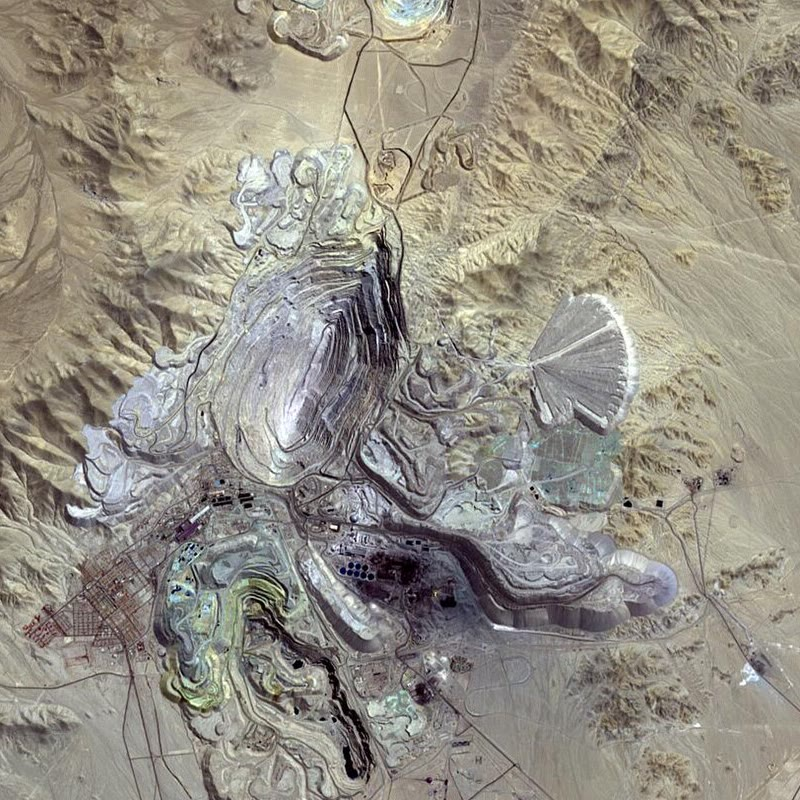
\includegraphics[width=\linewidth]{images/book1/g9-chuquicamata.jpg}
\end{minipage}\hfill
\begin{minipage}[c]{0.5\linewidth}\raggedright
{\small चिली के अटाकामा \omterm{def:g5:weather-and-climate:desert}{मरुस्थल} में चुकीकामाटा ताँबा खान, 2007 में NASA के एक उपग्रह
पर लगे ASTER उपकरण से देखी गई (चित्र लगभग \qty{12}{km} चौड़ा है)। बीच का अंडाकार
गड्ढा, जिसमें सौ वर्ष से ज़्यादा से खनन होता रहा है, \qty{4.3}{km} लंबा, \qty{2.7}{km}
चौड़ा और \qty{1.1}{km} गहरा है। NASA/METI/AIST/जापान स्पेस
सिस्टम्स और अमेरिका/जापान ASTER विज्ञान दल (सार्वजनिक डोमेन, विकिमीडिया
कॉमन्स के
ज़रिए)।}
\end{minipage}
% ledger: commons:chuquicamata, earle:chuquicamata
\label{fig:g9:earth-resources:chuquicamata}
\end{omfigure}

\paragraph{नदी की बजरी में।} सोने में जंग नहीं लगता और उसका \omterm{def:g5:water-shapes-the-land:weathering}{अपक्षय} मुश्किल से होता है।
जब \omterm{def:g5:water-shapes-the-land:erosion}{अपरदन} सोने की किसी शिरा को घिस देता है, तो सोना धूल, पपड़ियों, कणों और कभी-कभी डलों
के रूप में मुक्त होता है, और \omterm{def:g1:landscapes-around-us:water}{नदियाँ} उसे नीचे की ओर बहा ले जाती हैं। सोना बहुत सघन है: शुद्ध
रूप में लगभग \qty{19}{g/cm^3}, जबकि साधारण \omterm{def:g3:stones-pebbles-sand:rock}{चट्टान} का लगभग \qty{2.5}{g/cm^3}। \omterm{def:g5:water-shapes-the-land:flood}{बाढ़ों}
में, जब \omterm{def:g3:stones-pebbles-sand:sand}{रेत} और \omterm{def:g3:stones-pebbles-sand:pebble}{बजरी} का पूरा तल खिसकता है, तो सोने के भारी कण धीरे-धीरे नीचे पहुँचते हैं
और आधार-शैल पर इकट्ठा हो जाते हैं। भूवैज्ञानिक ऐसे निक्षेपों को
\emph{प्लेसर}\index{प्लेसर} कहते हैं।
% ledger: usgs:gold-placer

\section{कोयला, तेल और गैस}

कोयला, तेल और प्राकृतिक गैस जीवों के अवशेष हैं, जो सड़ने से पहले दब गए। किसी मृत पौधे या
जंतु का लगभग सारा कार्बनिक पदार्थ हफ़्तों से दशकों के भीतर वापस कार्बन डाइऑक्साइड में बदल
जाता है। केवल वह हिस्सा, जो हवा की ऑक्सीजन से कटा रहता है, किसी ठहरे दलदल या गहरे \omterm{def:g2:water-on-earth:ocean}{समुद्र}
के तल पर, दबकर लाखों वर्षों तक बचा रह सकता
है।
% ledger: earle:coal, earle:oil-gas

\begin{omfigure}
\begin{minipage}[c]{0.46\linewidth}\centering
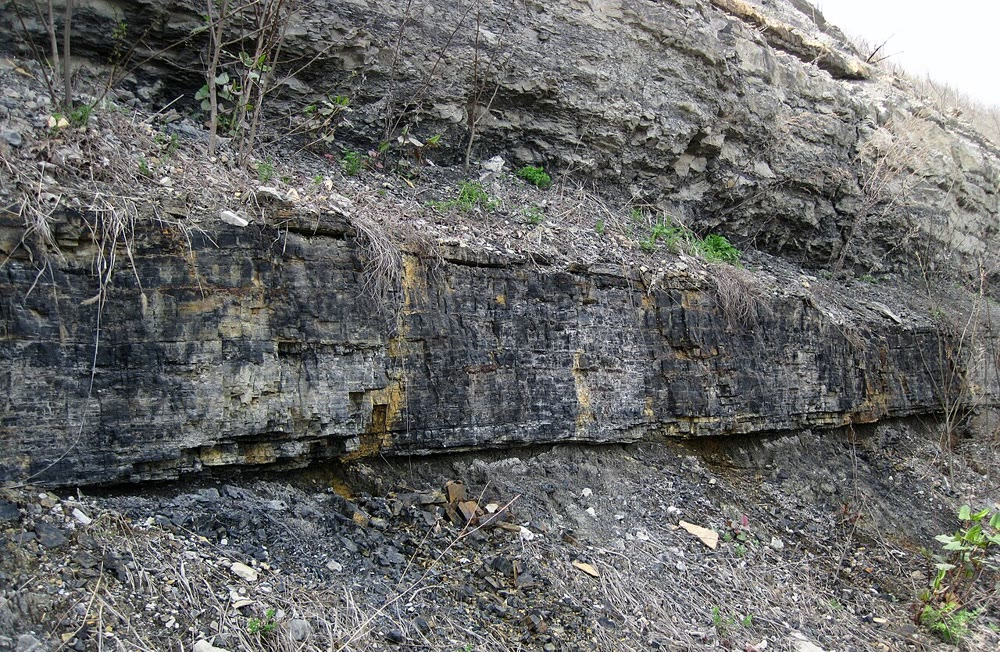
\includegraphics[width=\linewidth]{images/book1/g9-coal-seam.jpg}
\end{minipage}\hfill
\begin{minipage}[c]{0.5\linewidth}\raggedright
{\small कोयले की एक सीम, बीच में फैली गहरी परत, \omterm{def:g6:rocks-and-minerals:rock-families}{अवसादी चट्टानों} के बीच, संयुक्त
राज्य अमेरिका के ओहायो में एक सड़क के किनारे। सीम समतल पड़ी है, जैसे दलदल पड़ा था। फ़ोटो:
जेम्स सेंट~जॉन (CC BY 2.0, विकिमीडिया
कॉमन्स के ज़रिए)।}
\end{minipage}
% ledger: commons:meigs-coal
\label{fig:g9:earth-resources:coal-seam}
\end{omfigure}


\paragraph{कोयला।} कोयला \omterm{def:g1:landscapes-around-us:water}{नदियों} और \omterm{def:g5:water-shapes-the-land:delta}{डेल्टाओं} के बगल के दलदलों में, गरम और नम \omterm{def:g5:weather-and-climate:climate}{जलवायु} में,
शुरू होता है, जहाँ पौधे तेज़ी से उगते हैं। मरे हुए तने और पत्तियाँ ऐसे शांत पानी में गिरते हैं
जिसमें ऑक्सीजन कम होती है, और सड़ते नहीं। मोटी परत बनाने के लिए दलदल को सदियों से
सहस्राब्दियों तक बने रहना पड़ता है। एक दिन कोई \omterm{def:g1:landscapes-around-us:water}{नदी} रास्ता बदलती है या उफनती है, और दलदल को
\omterm{def:g3:stones-pebbles-sand:sand}{रेत} और \omterm{def:g3:stones-pebbles-sand:sand}{कीचड़} से ढक देती है। जैसे-जैसे और \omterm{def:g7:sediments-and-fossils:sediment}{अवसाद} जमा होते हैं, पौधों की परत दबती और गरम होती
है, और कोयले में बदल जाती है: पहले लगभग एक तिहाई कार्बन वाला एक मुलायम, भूरा कोयला, कुछ
सौ मीटर नीचे; 86~\% तक कार्बन वाला एक कठोर काला कोयला, कुछ किलोमीटर नीचे। उदाहरण के लिए,
संयुक्त राज्य अमेरिका में आज खोदा जाने वाला कोयला ज़्यादातर 100 से 300~मिलियन वर्ष पुराना
है।
% ledger: earle:coal, eia:coal

\begin{omfigure}
\begin{tikzpicture}[x=1cm, y=0.8cm, font=\footnotesize]
  \foreach \i/\t in {0/{(क) दलदली वन:\\ शांत पानी के नीचे\\ मरे पौधे जमा होते हैं},
                     1/{(ख) नदी की रेत और कीचड़\\ के नीचे दबकर परत\\ भिंच जाती है},
                     2/{(ग) और गहरी, और गरम\\ (सैकड़ों मीटर):\\ मुलायम भूरा कोयला},
                     3/{(घ) और भी गहरी\\ (किलोमीटर):\\ कठोर काला कोयला}} {
    \begin{scope}[xshift=\i*3.35cm]
      \draw[black!40] (0,0) rectangle (2.9,4.2);
      \node[align=center, anchor=north, font=\scriptsize] at (1.45,-0.1) {\t};
    \end{scope}
  }
  % (a) swamp: water, trees, plant layer
  \fill[omSea] (0,2.6) rectangle (2.9,3.1);
  \fill[brown!60!black!70] (0,2.0) rectangle (2.9,2.6);
  \fill[omLithShale] (0,0) rectangle (2.9,2.0);
  \foreach \x in {0.5,1.4,2.3} {
    \draw[brown!50!black, line width=1.2pt] (\x,2.6) -- (\x,3.7);
    \fill[green!45!black] (\x,3.85) circle (0.3);
  }
  % (b) buried
  \begin{scope}[xshift=3.35cm]
    \fill[lith sandstone] (0,2.6) rectangle (2.9,4.0);
    \fill[brown!55!black!80] (0,2.2) rectangle (2.9,2.6);
    \fill[omLithShale] (0,0) rectangle (2.9,2.2);
    \draw[->, thick] (1.45,4.15) -- (1.45,3.45);
  \end{scope}
  % (c) lignite
  \begin{scope}[xshift=6.7cm]
    \fill[lith sandstone] (0,1.9) rectangle (2.9,4.2);
    \fill[brown!45!black] (0,1.65) rectangle (2.9,1.9);
    \fill[omLithShale] (0,0) rectangle (2.9,1.65);
  \end{scope}
  % (d) coal
  \begin{scope}[xshift=10.05cm]
    \fill[lith sandstone] (0,1.25) rectangle (2.9,4.2);
    \fill[black!85] (0,1.1) rectangle (2.9,1.25);
    \fill[omLithShale] (0,0) rectangle (2.9,1.1);
  \end{scope}
\end{tikzpicture}

{\small दलदल से कोयले की सीम तक (एक रेखाचित्र, पैमाने पर नहीं)। जैसे-जैसे पौधों की परत
और गहरे धँसती है, वह दबती और गरम होती है: पानी और गैसें उसे छोड़ देती हैं, वह पतली होती
जाती है, और उसमें कार्बन का हिस्सा बढ़ता है।}
% ledger: earle:coal, eia:coal
\label{fig:g9:earth-resources:coal}
\end{omfigure}


\paragraph{तेल और गैस।} तेल और ज़्यादातर प्राकृतिक गैस \omterm{def:g2:water-on-earth:ocean}{समुद्र} में रहने वाले नन्हे पौधों
और जंतुओं से आते हैं, जैसे डायटम। उनके अवशेष \omterm{def:g3:stones-pebbles-sand:sand}{कीचड़} के साथ समुद्री तल पर डूब जाते हैं, और
कुछ सड़ने से पहले दब जाते हैं। लाखों वर्षों और किलोमीटरों \omterm{def:g7:sediments-and-fossils:sediment}{अवसाद} के बाद, ऊष्मा और दाब उन्हें
बदल देते हैं: लगभग \qty{2}{km} से नीचे, लगभग 60 और \qty{120}{\degreeCelsius} के बीच,
तेल में; और गरम होने पर, गैस में। तेल और गैस पानी से हल्के होते हैं। वे \omterm{def:g6:water-underground:permeability}{पारगम्य} \omterm{def:g3:stones-pebbles-sand:rock}{चट्टानों} के
छिद्रों से धीरे-धीरे ऊपर रिसते हैं, और बहुत-से सतह तक पहुँचकर खो जाते हैं। जो हमें मिलते
हैं, वे रास्ते में \omterm{def:g6:water-underground:permeability}{अपारगम्य} \omterm{def:g3:stones-pebbles-sand:rock}{चट्टान} की किसी परत से रुक गए थे, अक्सर ऊपर की ओर मुड़ी परतों के
किसी उभार के शिखर पर, जहाँ वे इकट्ठा होते हैं: सबसे ऊपर गैस, उसके नीचे तेल, और उसके नीचे
पानी।
% ledger: eia:oil, eia:gas, earle:oil-gas

\begin{omfigure}
\begin{tikzpicture}[x=1cm, y=1cm, font=\footnotesize, >={Stealth[length=2mm]}]
  \def\fold#1{(0,#1) .. controls (3,#1+1.0) and (4.0,#1+1.6) .. (6,#1+1.6) .. controls (8.0,#1+1.6) and (9,#1+1.0) .. (12,#1)}
  % layers from the bottom up
  \fill[omLithShale!60!black!40] (0,0) -- \fold{0.9} -- (12,0) -- cycle;
  \fill[lith sandstone] \fold{0.9} -- (12,2.1) -- (12,2.1) .. controls (9,3.1) and (8.0,3.7) .. (6,3.7) .. controls (4.0,3.7) and (3,3.1) .. (0,2.1) -- cycle;
  \fill[lith shale] (0,2.1) .. controls (3,3.1) and (4.0,3.7) .. (6,3.7) .. controls (8.0,3.7) and (9,3.1) .. (12,2.1) -- (12,3.6) .. controls (9,4.6) and (8.0,5.2) .. (6,5.2) .. controls (4.0,5.2) and (3,4.6) .. (0,3.6) -- cycle;
  \fill[lith sandstone] (0,3.6) .. controls (3,4.6) and (4.0,5.2) .. (6,5.2) .. controls (8.0,5.2) and (9,4.6) .. (12,3.6) -- (12,5.6) -- (0,5.6) -- cycle;
  % gas and oil under the crest of the impermeable layer
  \fill[omWxSun!60] (4.55,3.55) .. controls (5.2,3.69) and (6.8,3.69) .. (7.45,3.55) -- (7.1,3.35) -- (4.9,3.35) -- cycle;
  \fill[black!75] (4.9,3.35) -- (7.1,3.35) -- (8.05,3.05) .. controls (7.0,3.15) and (5.0,3.15) .. (3.95,3.05) -- cycle;
  % arrows: oil creeping up through the permeable layer
  \draw[->, black, thick] (1.4,2.05) -- (2.4,2.55);
  \draw[->, black, thick] (10.6,2.05) -- (9.6,2.55);
  \draw[->, black!70] (3.0,2.65) -- (3.8,2.95);
  \draw[->, black!70] (9.0,2.65) -- (8.2,2.95);
  % labels
  \node[anchor=west, fill=white, fill opacity=0.85, text opacity=1, inner sep=1.5pt] at (0.1,0.45) {पुराने समुद्री तल का गहरा कीचड़: तेल और गैस यहाँ बनते हैं};
  \node[anchor=east, fill=white, fill opacity=0.85, text opacity=1, inner sep=1.5pt] at (11.9,1.9) {पारगम्य बलुआ पत्थर};
  \node[anchor=east, fill=white, fill opacity=0.85, text opacity=1, inner sep=1.5pt] at (11.9,3.25) {अपारगम्य शेल};
  \node[anchor=south, fill=white, fill opacity=0.85, text opacity=1, inner sep=1.5pt] at (6,5.25) {सतह की चट्टानें};
  \node[font=\scriptsize] at (6,3.48) {गैस};
  \node[font=\scriptsize, text=white] at (6,3.22) {तेल};
\end{tikzpicture}

{\small किसी उभार के शिखर पर एक \omterm{def:g6:water-underground:permeability}{अपारगम्य} परत के नीचे रुके तेल और गैस (एक रेखाचित्र,
पैमाने पर नहीं; बलुआ पत्थर के बाक़ी हिस्से को भरने वाला पानी नहीं दिखाया गया है)। मोड़ के नीचे
वे \omterm{def:g6:water-underground:permeability}{पारगम्य} बलुआ पत्थर से ऊपर रिसते हैं (तीर) और शिखर के नीचे इकट्ठा होते हैं: ऊपर गैस,
नीचे
तेल।}
% ledger: earle:oil-gas
\label{fig:g9:earth-resources:oil}
\end{omfigure}

\section{ज़मीन से पानी}

\omterm{def:g6:water-underground:groundwater}{भूजल} भी पृथ्वी से मिलने वाला एक संसाधन है, वह जिसका हम हर दिन उपयोग करते हैं। किसी धातु
या कोयले के विपरीत, वह फिर से बनता है: \omterm{def:g4:clouds-rain-snow:precipitation}{बारिश} \omterm{def:g6:water-underground:aquifer}{जलभृतों} को फिर से भरती है। पर वह धीरे-धीरे
फिर से बनता है, और केवल उतनी ही तेज़ी से जितनी तेज़ी से \omterm{def:g4:clouds-rain-snow:precipitation}{बारिश} रिसकर अंदर जाती है। जिस \omterm{def:g6:water-underground:aquifer}{जलभृत}
से उसके भरने से ज़्यादा तेज़ी से पानी खींचा जाए, उसका \omterm{def:g6:water-underground:water-table}{भौम जलस्तर} गिरता है, और \omterm{def:g6:water-underground:spring}{कुएँ} सूख जाते
हैं (\cref{ch:g6:water-underground})। \omterm{def:g6:water-underground:groundwater}{भूजल} तभी तक नवीकरणीय संसाधन है जब तक उसे उसके
फिर से बनने से ज़्यादा तेज़ी से न खींचा जाए।
% ledger: wss:aquifer

\section{रेत और बजरी}

लोग ज़मीन से जो ठोस पदार्थ सबसे बड़ी मात्रा में खोदकर निकालते हैं, वह न कोयला है न कोई
धातु अयस्क: वह \omterm{def:g3:stones-pebbles-sand:sand}{रेत} और \omterm{def:g3:stones-pebbles-sand:pebble}{बजरी} है।
% ledger: tos:sand

\begin{definition}[समुच्चय]\label{def:g9:earth-resources:aggregate}
\emph{समुच्चय}\index{समुच्चय} निर्माण में इस्तेमाल होने वाली \omterm{def:g3:stones-pebbles-sand:sand}{रेत}, \omterm{def:g3:stones-pebbles-sand:pebble}{बजरी} और कुचला
पत्थर हैं: कंक्रीट में, सड़कों और रेल पटरियों के नीचे, और ज़मीन भरने के
लिए।
\end{definition}
% ledger: usgs:aggregate, tos:sand

ज़्यादातर \omterm{def:g3:stones-pebbles-sand:sand}{रेत} कंक्रीट में जाती है, जो \omterm{def:g3:stones-pebbles-sand:sand}{रेत}, \omterm{def:g3:stones-pebbles-sand:pebble}{बजरी}, पानी और सीमेंट का मिश्रण है। 2019 में दुनिया
को हर वर्ष लगभग 50~अरब टन \omterm{def:g3:stones-pebbles-sand:sand}{रेत} और \omterm{def:g3:stones-pebbles-sand:pebble}{बजरी} की ज़रूरत थी, यानी $5 \times 10^{10}$ टन, या
पृथ्वी पर हर व्यक्ति के लिए, हर दिन, लगभग \qty{18}{kg}। \omterm{def:g3:stones-pebbles-sand:sand}{रेत} और \omterm{def:g3:stones-pebbles-sand:pebble}{बजरी} ज़मीन पर के गड्ढों
से, \omterm{def:g1:landscapes-around-us:water}{नदी} तलों से और, बढ़ती मात्रा में, समुद्री तल से खोदी जाती है। \omterm{def:g1:landscapes-around-us:water}{नदी} से ली जाने पर \omterm{def:g1:landscapes-around-us:water}{तट} तक
पहुँचने के लिए कम \omterm{def:g3:stones-pebbles-sand:sand}{रेत} बचती है, और नीचे की ओर के \omterm{def:g2:water-on-earth:ocean}{समुद्र} \omterm{def:g1:landscapes-around-us:water}{तट} घिसकर छोटे होते
हैं।
% ledger: tos:sand

\begin{omfigure}
\begin{minipage}[c]{0.46\linewidth}\centering
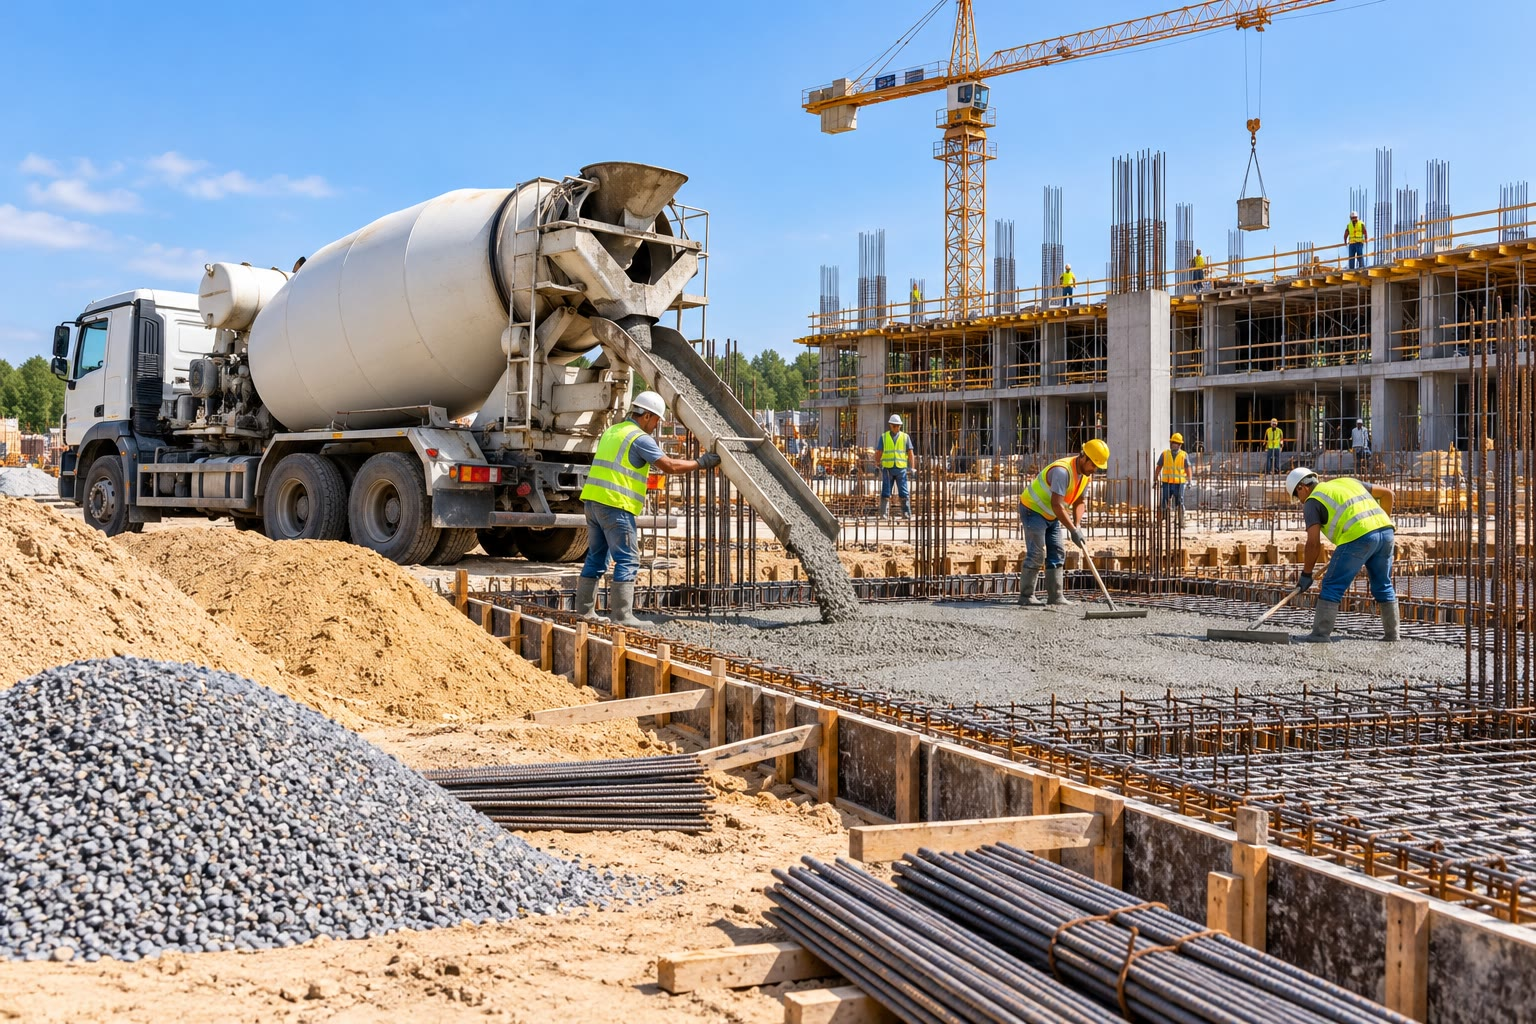
\includegraphics[width=\linewidth]{images/book1/ai/g9-building-site.jpg}
\end{minipage}\hfill
\begin{minipage}[c]{0.5\linewidth}\raggedright
{\small काम में लगे \omterm{def:g9:earth-resources:aggregate}{समुच्चय}: एक नई इमारत का फ़र्श ढालते कंक्रीट मिक्सर ट्रक के बगल में
\omterm{def:g3:stones-pebbles-sand:sand}{रेत} और \omterm{def:g3:stones-pebbles-sand:pebble}{बजरी} के ढेर (एक सामान्य दृश्य का AI
चित्रण)।}
\end{minipage}
\label{fig:g9:earth-resources:building-site}
\end{omfigure}

\section{नवीकरणीय या सीमित?}

कोई संसाधन जिसे प्रकृति एक मानव जीवनकाल के भीतर फिर से बना देती है, जैसे किसी ऐसे \omterm{def:g6:water-underground:aquifer}{जलभृत}
का पानी जिससे ज़्यादा पानी न खींचा जाए, हमेशा इस्तेमाल किया जा सकता है। किसी \omterm{def:g9:earth-resources:ore-deposit}{अयस्क निक्षेप},
कोयले की सीम या तेल क्षेत्र को बनने में लाखों वर्ष लगे। हम उसे कुछ दशकों में इस्तेमाल कर
लेते हैं: हमारे समय-पैमाने पर वह बिलकुल फिर से नहीं बनता।
% ledger: eia:coal, earle:coal

\begin{omfigure}
\begin{tikzpicture}
\begin{axis}[xmode=log, width=12.5cm, height=4.6cm, xmin=10, xmax=1e9, ymin=0.4, ymax=4.6,
  ytick=\empty, xlabel={वर्ष (लघुगणकीय पैमाना)}, label style={font=\small},
  xtick={10,100,1000,1e4,1e5,1e6,1e7,1e8,1e9},
  xticklabels={$10$,$10^2$,$10^3$,$10^4$,$10^5$,$10^6$,$10^7$,$10^8$,$10^9$},
  tick label style={font=\footnotesize}, xmajorgrids, grid style={black!12}, clip=false]
\addplot[only marks, mark=|, mark size=4pt, line width=4pt, omWarm,
  error bars/.cd, x dir=plus, x explicit, error bar style={line width=4pt, omWarm}, error mark=none]
  table[x=lo_yr, y=y, x error expr=\thisrow{hi_yr}-\thisrow{lo_yr}] {figdata/out/grade-9-concentration-times.dat};
\node[anchor=west, font=\footnotesize, fill=white, inner sep=1pt] at (axis cs:1500,4) {दलदल पौधों की मोटी परत बनाता है};
\node[anchor=east, font=\footnotesize, fill=white, inner sep=1pt] at (axis cs:6e7,3) {अमेरिका में खोदे जाने वाले कोयले की आयु};
\node[anchor=west, font=\footnotesize, fill=white, inner sep=1pt] at (axis cs:150,2) {चुकीकामाटा में अब तक खनन (सौ वर्ष से ज़्यादा)};
\node[anchor=west, font=\footnotesize, fill=white, inner sep=1pt] at (axis cs:65,1) {2024 की खनन दर पर दुनिया के ताँबा भंडार};
\end{axis}
\end{tikzpicture}

{\small बनने के समय और इस्तेमाल के समय, ऐसे पैमाने पर जहाँ हर क़दम पिछले क़दम का दस गुना
है। कोयला उस समय से लगभग दस लाख गुना पुराना है जो किसी खान को एक निक्षेप ख़ाली करने में
लगता है।}
% ledger: earle:coal, eia:coal, earle:chuquicamata, usgs:mcs-copper (figdata/grade-9/concentration.py, part times)
\label{fig:g9:earth-resources:times}
\end{omfigure}

कोई संसाधन कितने समय तक चलेगा? भूवैज्ञानिक केवल उसे गिनते हैं जो ज्ञात है और निकाला जा
सकता है।

\begin{definition}[भंडार]\label{def:g9:earth-resources:reserve}
किसी \omterm{def:g6:rocks-and-minerals:mineral}{खनिज} संसाधन का \emph{भंडार}\index{भंडार} ज्ञात निक्षेपों का वह हिस्सा है जिसे उस समय
की तकनीकों और क़ीमतों पर मुनाफ़े के साथ निकाला जा
सकता है।
\end{definition}
% ledger: usgs:mcs-reserves

\omterm{def:g9:earth-resources:reserve}{भंडार} वह सब नहीं है जो ज़मीन में है। वह तब बढ़ता है जब नए निक्षेप मिलते हैं, जब तकनीकें
सुधरती हैं या जब क़ीमतें बढ़ती हैं, और निक्षेपों के खनन के साथ घटता है। 1970 में दुनिया के
ताँबा \omterm{def:g9:earth-resources:reserve}{भंडारों} का अनुमान 280~मिलियन टन लगाया गया था। तब से लगभग 700~मिलियन टन ताँबा खोदा
जा चुका है, उस \omterm{def:g9:earth-resources:reserve}{भंडार} का ढाई गुना, और फिर भी 2024 के \omterm{def:g9:earth-resources:reserve}{भंडारों} का अनुमान 980~मिलियन टन लगाया
गया।
% ledger: usgs:mcs-reserves

\begin{dated}{2025}
2024 में दुनिया की खानों ने लगभग 23~मिलियन टन ताँबा पैदा किया। उस दर पर 980~मिलियन टन के
\omterm{def:g9:earth-resources:reserve}{भंडार} $980 \div 23
\approx 43$ वर्ष चलेंगे। ऐसी संख्या कोई तारीख़ नहीं है जब ताँबा ख़त्म
हो जाएगा: वह उस ताँबे का एक माप है जो आज ज्ञात है और निकालने लायक़
है।
\end{dated}
% ledger: usgs:mcs-copper (figdata/grade-9/concentration.py: 42.6 years)

कोई धातु, कोयले या तेल के विपरीत, इस्तेमाल होने पर नष्ट नहीं होती: पदार्थों का
पुनर्चक्रण, जिससे तुम रसायन विज्ञान की किताबों में मिलते हो, उसे वापस दे देता है। किसी पुराने
तार का, कबाड़ हुए इंजन का या किसी कारख़ाने की कतरनों का ताँबा फिर से पिघलाया और शुद्ध किया
जा सकता है। 2024 में संयुक्त राज्य अमेरिका में कबाड़ से वापस पाया गया ताँबा इस्तेमाल हुए
सारे ताँबे का लगभग \qty{35}{\%}
था।
% ledger: usgs:mcs-copper-scrap

\begin{omfigure}
\begin{tikzpicture}[font=\footnotesize, node distance=1.2cm,
  box/.style={draw=black!60, fill=black!4, rounded corners=2pt, align=center, minimum height=0.9cm, inner sep=3pt},
  flow/.style={-{Stealth[length=2.2mm]}, line width=0.9pt, black!70}]
  \node[box, fill=omWarm!12] (ore) at (0,0) {अयस्क निक्षेप\\(\qty{0.5}{\%} ताँबे\\वाली चट्टान)};
  \node[box] (metal) at (4.2,0) {ताँबा धातु};
  \node[box] (things) at (8.2,0) {तार, पाइप,\\इंजन};
  \node[box, fill=blue!8] (scrap) at (6.2,-2.1) {कबाड़};
  \node[box, fill=black!12] (waste) at (0,-2.1) {बची हुई\\कुचली चट्टान};
  \draw[flow] (ore) -- node[above] {खोदना, कुचलना,} node[below] {सांद्रित करना} (metal);
  \draw[flow] (metal) -- node[above] {बनाना} (things);
  \draw[flow] (things) |- node[pos=0.25, right] {फेंक दिया} (scrap);
  \draw[flow] (scrap) -| node[pos=0.75, left] {पिघलाना, शुद्ध करना} (metal);
  \draw[flow] (ore) -- (waste);
\end{tikzpicture}

{\small ताँबा धातु तक के दो रास्ते: अयस्क से, टनों खोदी और कुचली गई \omterm{def:g3:stones-pebbles-sand:rock}{चट्टान} से होकर, या
कबाड़ से, जिसे फिर से पिघलाया और शुद्ध किया जाता है।}
\end{omfigure}

\begin{example}[वह चट्टान जो पुनर्चक्रण बचाता है]\label{ex:g9:earth-resources:recycling}
\qty{0.5}{\%} ताँबे वाले अयस्क में हर टन \omterm{def:g3:stones-pebbles-sand:rock}{चट्टान} में \qty{5}{kg} ताँबा होता है। एक टन ताँबा
बनाने के लिए लगभग $1000 \div 5 = 200$ टन अयस्क खोदना, कुचलना और उपचारित करना पड़ता है,
और उसका लगभग सारा हिस्सा बेकार \omterm{def:g3:stones-pebbles-sand:rock}{चट्टान} बनकर रह जाता है। कबाड़ से बना हर टन ताँबा वे 200
टन \omterm{def:g3:stones-pebbles-sand:rock}{चट्टान} ज़मीन में छोड़ देता है --- और निक्षेप ज़्यादा समय तक चलता
है।
% ledger: perkins:ore-grades (computed)
\end{example}


\section{अभ्यास}

\begin{exercise}[$\star$]\label{exo:g9:earth-resources:1}
सही शब्द से पूरा करो (\omterm{def:g9:earth-resources:ore-deposit}{अयस्क निक्षेप}, \omterm{def:g9:earth-resources:ore-deposit}{सांद्रण गुणक}, \omterm{def:g9:earth-resources:aggregate}{समुच्चय}, \omterm{def:g9:earth-resources:reserve}{भंडार})। (क) कंक्रीट में इस्तेमाल
होने वाली \omterm{def:g3:stones-pebbles-sand:sand}{रेत} एक \ldots\ है। (ख) ज्ञात ताँबे का वह हिस्सा जिसे आज मुनाफ़े के साथ निकाला जा
सकता है, ताँबे का \ldots\ है। (ग) ऐसी \omterm{def:g3:stones-pebbles-sand:rock}{चट्टान} जिसमें कोई धातु खनन लायक़ समृद्ध हो, एक
\ldots\ है। (घ) कोई धातु जितनी बार सांद्रित हुई है, वह संख्या उसका \ldots\ है।
\end{exercise}

\begin{exercise}[$\star$]\label{exo:g9:earth-resources:2}
% ledger: earle:magmatic, usgs:gold-lode, usgs:gold-placer
हर वाक्य किसी धातु को सांद्रित करने के किस तरीक़े का वर्णन करता है: \omterm{def:g7:volcanoes:magma}{मैग्मा} में, दरारों में
गरम पानी से, या \omterm{def:g1:landscapes-around-us:water}{नदी} की \omterm{def:g3:stones-pebbles-sand:pebble}{बजरी} में? (क) किसी धारा की \omterm{def:g3:stones-pebbles-sand:pebble}{बजरी} के नीचे आधार-शैल पर सोने के डले
पड़े हैं। (ख) गरम पानी एक दरार को क्वार्ट्ज़ और सोने से भर देता है। (ग) एक पुराने \omterm{def:g7:volcanoes:magma}{मैग्मा}
पिंड के तल में भारी निकल \omterm{def:g6:rocks-and-minerals:mineral}{खनिजों} की एक परत है। (घ) \omterm{def:g5:water-shapes-the-land:erosion}{अपरदन} से सोना एक शिरा से मुक्त होता
है।
\end{exercise}

\begin{exercise}[$\star$]\label{exo:g9:earth-resources:3}
% ledger: earle:coal, eia:coal
इन चरणों को क्रम में रखो: (क) पौधों की परत \omterm{def:g1:landscapes-around-us:water}{नदी} की \omterm{def:g3:stones-pebbles-sand:sand}{रेत} के नीचे दब जाती है;
(ख) एक दलदल में पेड़ उगते हैं; (ग) किलोमीटरों नीचे एक कठोर काला कोयला बनता है;
(घ) मरे पौधे शांत पानी के नीचे जमा होते हैं; (ङ) एक मुलायम भूरा कोयला बनता है।
\end{exercise}

\begin{exercise}[$\star$]\label{exo:g9:earth-resources:4}
एक मानव जीवन के पैमाने पर हर संसाधन नवीकरणीय है या नहीं? एक वाक्य में समझाओ।
(क) कोयला। (ख) ऐसे \omterm{def:g6:water-underground:aquifer}{जलभृत} का पानी जिससे \omterm{def:g4:clouds-rain-snow:precipitation}{बारिश} के भरने से कम पानी खींचा जाता है। (ग) ताँबे
का अयस्क। (घ) वही \omterm{def:g6:water-underground:aquifer}{जलभृत}, जिससे उसके भरने से दोगुनी तेज़ी से पानी खींचा
जाता है।
\end{exercise}

\begin{exercise}[$\star\star$]\label{exo:g9:earth-resources:5}
% ledger: perkins:ore-grades
\omterm{def:g9:earth-resources:ore-deposit}{सांद्रण गुणक} निकालो, फिर उसे पूर्णांकित करके दस की घात के रूप में लिखो:
(क) जस्ता, \omterm{def:g6:inside-the-earth:layers}{भूपर्पटी} में \qty{0.007}{\%}, अयस्क \qty{4}{\%} से; (ख) टिन,
\omterm{def:g6:inside-the-earth:layers}{भूपर्पटी} में \qty{0.0002}{\%}, अयस्क \qty{0.5}{\%} से; (ग) लोहा,
\omterm{def:g6:inside-the-earth:layers}{भूपर्पटी} में \qty{5.6}{\%}, अयस्क \qty{20}{\%} से। (घ) लोहे को इतने कम सांद्रण की ज़रूरत
क्यों होती है?
\end{exercise}

\begin{exercise}[$\star\star$]\label{exo:g9:earth-resources:6}
% ledger: usgs:gold-placer
शुद्ध सोने का घनत्व लगभग \qty{19.3}{g/cm^3} है; साधारण \omterm{def:g3:stones-pebbles-sand:rock}{चट्टान} का लगभग
\qty{2.5}{g/cm^3}। (क) सोना कितने गुना ज़्यादा सघन है? (ख) \qty{0.01}{cm^3} के सोने
के कण का द्रव्यमान क्या है, और उसी आकार के \omterm{def:g3:stones-pebbles-sand:rock}{चट्टान} के कण का? (ग) समझाओ कि \omterm{def:g5:water-shapes-the-land:flood}{बाढ़} में सोना
\omterm{def:g3:stones-pebbles-sand:pebble}{बजरी} के तल में, आधार-शैल पर, क्यों पहुँच जाता
है।
\end{exercise}

\begin{exercise}[$\star\star$]\label{exo:g9:earth-resources:7}
% ledger: perkins:ore-grades, earle:ore-grades (figdata/grade-9/concentration.py)
\omterm{def:g9:earth-resources:ore-deposit}{सांद्रण गुणकों} वाले चार्ट का उपयोग करो। (क) किन धातुओं को $10^3$ से ज़्यादा गुणक की ज़रूरत
है? (ख) ताँबा दस की किन घातों के बीच है? (ग) क्रोमियम को एल्युमिनियम से कितने गुना ज़्यादा
सांद्रित होना पड़ता है? (घ) सात धातुओं में से किसके सबसे कम जगहों पर खोदे जाने की तुम उम्मीद
करोगे? समझाओ।
\end{exercise}

\begin{exercise}[$\star\star$]\label{exo:g9:earth-resources:8}
% ledger: tos:sand
दुनिया को प्रति व्यक्ति प्रति दिन लगभग \qty{18}{kg} \omterm{def:g3:stones-pebbles-sand:sand}{रेत} और \omterm{def:g3:stones-pebbles-sand:pebble}{बजरी} चाहिए। (क) एक वर्ष में
प्रति व्यक्ति यह टन में कितना है? (ख) 50 अरब टन को वैज्ञानिक संकेतन में लिखो।
(ग) एक ट्रक \qty{25}{t} ढोता है। एक व्यक्ति के हिस्से से उसे भरने में कितने दिन लगते
हैं? (घ) \omterm{def:g1:landscapes-around-us:water}{नदी} से \omterm{def:g3:stones-pebbles-sand:sand}{रेत} लेने से नीचे की ओर का कोई \omterm{def:g2:water-on-earth:ocean}{समुद्र} \omterm{def:g1:landscapes-around-us:water}{तट} क्यों सिकुड़ सकता
है?
\end{exercise}

\begin{exercise}[$\star\star$]\label{exo:g9:earth-resources:9}
% ledger: earle:oil-gas, eia:oil
(क) ज़्यादातर तेल और गैस किन जीवों से आते हैं? (ख) लगभग \qty{2}{km} से नीचे, तेल
किन तापमानों पर बनता है? (ग) तेल और गैस \omterm{def:g3:stones-pebbles-sand:rock}{चट्टानों} में से ऊपर की ओर क्यों खिसकते हैं?
(घ) किस तरह की \omterm{def:g3:stones-pebbles-sand:rock}{चट्टान} उन्हें रोकती है, और वे कहाँ इकट्ठा होते
हैं?
\end{exercise}

\begin{exercise}[$\star\star$]\label{exo:g9:earth-resources:10}
% ledger: earle:chuquicamata
चुकीकामाटा खान ने 100 से ज़्यादा वर्षों में 29~मिलियन टन से ज़्यादा ताँबा पैदा किया है।
(क) 29~मिलियन टन को वैज्ञानिक संकेतन में लिखो। (ख) प्रति वर्ष औसत उत्पादन मोटे तौर
पर कितना है? (ग) अगर अयस्क में \qty{1}{\%} ताँबा होता, तो 29~मिलियन टन ताँबा पाने के
लिए कितने टन अयस्क खोदा गया? वैज्ञानिक संकेतन का उपयोग करो। (घ) इतने कमज़ोर अयस्क की खान
को इतना बड़ा क्यों होना पड़ता
है?
\end{exercise}

\begin{exercise}[$\star\star\star$]\label{exo:g9:earth-resources:11}
% ledger: usgs:mcs-reserves, usgs:mcs-copper
1970 में दुनिया के ताँबा \omterm{def:g9:earth-resources:reserve}{भंडारों} का अनुमान 280~मिलियन टन लगाया गया था। 1970 से 2024
तक लगभग 697~मिलियन टन खोदा गया, और 2024 के \omterm{def:g9:earth-resources:reserve}{भंडार} 980~मिलियन टन थे, जबकि 2024 में
23~मिलियन टन खोदा गया। (क) अगर 1970 का \omterm{def:g9:earth-resources:reserve}{भंडार} ही सारा ताँबा होता, तो वह कब ख़त्म हो
जाता? खोदे गए ताँबे से तुलना करो। (ख) 2024 का \omterm{def:g9:earth-resources:reserve}{भंडार} 1970 वाले से कितने गुना बड़ा है?
(ग) निकालो कि 2024 का \omterm{def:g9:earth-resources:reserve}{भंडार} 2024 की दर पर कितने वर्ष चलेगा। (घ) दो कारण बताओ कि
खनन होते रहने पर भी कोई \omterm{def:g9:earth-resources:reserve}{भंडार} क्यों बढ़ सकता
है।
\end{exercise}

\begin{exercise}[$\star\star\star$]\label{exo:g9:earth-resources:12}
% ledger: earle:coal, eia:coal
कोयले की एक सीम $3 \times 10^8$ वर्ष पुरानी है। उसका दलदल $2 \times 10^3$
वर्ष तक बना रहा, और सीम का खनन 50 वर्षों में पूरा हो जाता है। (क) 50 वर्ष को वैज्ञानिक
संकेतन में लिखो। (ख) दलदल खनन से कितने गुना ज़्यादा समय तक बना रहा? (ग) सीम खनन के
समय से कितने गुना पुरानी है? (घ) इन संख्याओं से समझाओ कि कोयले को अनवीकरणीय संसाधन
क्यों कहा जाता है।
\end{exercise}

\section{समस्या: एक नए नगर के लिए कंक्रीट}

\begin{problem}[{सप्ताहांत समस्या --- एक नया नगर एक स्थानीय गड्ढे की रेत से बनाया जाता है;
अंतिम उत्तर उन वर्षों की संख्या है जितने गड्ढे का रेत भंडार
चलेगा}]
\label{pb:g9:earth-resources:1}
% ledger: usgs:aggregate (about 100 and 300 t per home), tos:sand (figdata/grade-9/concentration.py, part problem: exercise data)
\num{2000} घरों का एक नया नगर दस वर्षों में बनना है, एक पुराने \omterm{def:g3:stones-pebbles-sand:sand}{रेत} के गड्ढे के पास, जो
किसी \omterm{def:g1:landscapes-around-us:water}{नदी} वेदिका की \omterm{def:g3:stones-pebbles-sand:pebble}{बजरी} में खोदा गया है। गलियों, स्कूलों और दुकानों में अपने हिस्से को गिनकर,
हर घर को लगभग \qty{300}{t} \omterm{def:g9:earth-resources:aggregate}{समुच्चय} की ज़रूरत है, जिसका \qty{40}{\%} \omterm{def:g3:stones-pebbles-sand:sand}{रेत} है। गड्ढे की
\omterm{def:g3:stones-pebbles-sand:sand}{रेत} की परत \qty{1.2}{km} लंबी, \qty{500}{m} चौड़ी और \qty{5}{m} मोटी है; उसकी एक
घन मीटर \omterm{def:g3:stones-pebbles-sand:sand}{रेत} का द्रव्यमान \qty{1.6}{t} है। गड्ढा क्षेत्र के बाक़ी हिस्से को हर वर्ष
\num{136000} टन \omterm{def:g3:stones-pebbles-sand:sand}{रेत} भी बेचता
है।

\noindent\textbf{भाग I --- कितनी रेत?}\par\nopagebreak
\begin{enumerate}[beginpenalty=10000]
  \item अकेले एक पारिवारिक घर को लगभग \qty{100}{t} \omterm{def:g9:earth-resources:aggregate}{समुच्चय} चाहिए। इस द्रव्यमान को
        किलोग्राम में, वैज्ञानिक संकेतन में, लिखो।
  \item पूरे नगर को कितने टन \omterm{def:g9:earth-resources:aggregate}{समुच्चय} की ज़रूरत होगी?
  \item दस वर्षों में यह प्रति वर्ष कितने टन है?
  \item नगर को प्रति वर्ष कितने टन \omterm{def:g3:stones-pebbles-sand:sand}{रेत} की ज़रूरत है?
\end{enumerate}

\noindent\textbf{भाग II --- भंडार।}\par\nopagebreak
\begin{enumerate}[resume, beginpenalty=10000]
  \item \omterm{def:g3:stones-pebbles-sand:sand}{रेत} की परत का आयतन घन मीटर में, वैज्ञानिक संकेतन में,
        निकालो।
  \item परत का एक तिहाई हिस्सा एक गाँव और एक सड़क के नीचे है और खोदा नहीं जाएगा।
        कितना आयतन निकाला जा सकता है?
  \item इस \omterm{def:g9:earth-resources:reserve}{भंडार} का द्रव्यमान टन में क्या है?
  \item गड्ढा नगर को और क्षेत्र को मिलाकर हर वर्ष कितने टन \omterm{def:g3:stones-pebbles-sand:sand}{रेत} बेचेगा?
\end{enumerate}

\noindent\textbf{भाग III --- नवीकरणीय या नहीं?}\par\nopagebreak
\begin{enumerate}[resume, beginpenalty=10000]
  \item हर वर्ष \omterm{def:g1:landscapes-around-us:water}{नदी} उस इलाक़े में लगभग \num{2000} टन नई \omterm{def:g3:stones-pebbles-sand:sand}{रेत} लाती है। गड्ढा कितने गुना
        ज़्यादा \omterm{def:g3:stones-pebbles-sand:sand}{रेत} बेचता है?
  \item नगर के जीवन के पैमाने पर, क्या यह \omterm{def:g3:stones-pebbles-sand:sand}{रेत} एक नवीकरणीय संसाधन है? समझाओ।
  \item अगर नगर अपनी \omterm{def:g3:stones-pebbles-sand:sand}{रेत} के एक चौथाई की जगह कुचला हुआ पुराना कंक्रीट इस्तेमाल करे, तो वह
        हर वर्ष कितने टन \omterm{def:g3:stones-pebbles-sand:sand}{रेत} बचाएगा?
  \item उस पुनर्चक्रण के बिना गड्ढे का \omterm{def:g3:stones-pebbles-sand:sand}{रेत} \omterm{def:g9:earth-resources:reserve}{भंडार} कितने वर्ष चलेगा?
\end{enumerate}
\end{problem}
